% Created 2020-04-09 Thu 17:15
% Intended LaTeX compiler: pdflatex
\documentclass[11pt]{article}
\usepackage[utf8]{inputenc}
\usepackage[T1]{fontenc}
\usepackage{graphicx}
\usepackage{grffile}
\usepackage{longtable}
\usepackage{wrapfig}
\usepackage{rotating}
\usepackage[normalem]{ulem}
\usepackage{amsmath}
\usepackage{textcomp}
\usepackage{amssymb}
\usepackage{capt-of}
\usepackage{hyperref}
\usepackage{minted}
\author{Lucas Michel Todó}
\date{31/03/2020}
\title{Creation of active gene-lists}
\hypersetup{
 pdfauthor={Lucas Michel Todó},
 pdftitle={Creation of active gene-lists},
 pdfkeywords={},
 pdfsubject={},
 pdfcreator={Emacs 26.3 (Org mode 9.1.9)},
 pdflang={English}}
\begin{document}

\maketitle
\tableofcontents \clearpage
\section{Actiev/Inactive Gene Lists}
\label{sec:org750967f}
Our aim is to create a unified table that assigns to each gene in the P.falicparum gnome a expresion state.
We will define 4 possible expresion states:
\begin{itemize}
\item Active
\begin{itemize}
\item Regular
\item Variant Active
\item Variant Repressed
\end{itemize}
\item Inactive
\end{itemize}

\subsection{Create microarrays DF}
\label{sec:org4c7774d}
We load our microarray data.
We willl load the red signal and transform it into percentiles.
We will also load the areas data to calculate FC among strains.

Red Signal DataFrame
\begin{verbatim}
              Gene_id     Red_12B     Red_10G    Red_3D7B Percent_12B
1          mal_mito_3 22579.33333 36436.73333 30636.82500  96.0335622
2 MAL13P1.415_oldname   770.82083   702.22292   640.11667  21.3196034
3  MAL13P1.65_oldname   111.33333    87.05833    91.05833   6.2166285
4  MAL7P1.142_oldname  5924.44167  5194.40000  5114.63333  75.4767353
5  MAL8P1.310_oldname    37.21250    35.37917    33.24167   0.8581236
6   MAL8P1.90_oldname    80.55417    46.18333    54.64167   4.1952708
  Percent_10G Percent_3D7B
1   98.474447   97.8832952
2   20.861937   18.4591915
3    5.053394    4.5194508
4   72.444699   71.7200610
5    1.115561    0.5911518
6    2.002288    2.2501907
\end{verbatim}

Areas DataFrame
\begin{verbatim}
               Old_id    l_12B     r_12B     m_12B    s_12B     l_10G    r_10G
1 1396.pre-tRNA-Met-1 52.07122 26.697018 48.027987 30.74025 48.007175 22.34826
2 1399.pre-tRNA-Gly-1 43.06044 27.673743 39.081224 31.65296 40.745787 20.85755
3 1399.pre-tRNA-Leu-1 41.86042 22.593902 35.842097 28.61222 41.137203 20.33420
4 1400.pre-tRNA-Gln-1 11.50002  9.748608  7.973428 13.27520  9.792214 10.93704
5 2277.pre-tRNA-Glu-1 52.29683 38.632652 46.014786 44.91469 50.436455 40.25664
6          mal_mito_3 30.59250 61.080128 49.676556 41.99607 25.372470 62.38873
      m_10G    s_10G    l_3D7B   r_3D7B    m_3D7B   s_3D7B MaxArea_12B
1 45.311433 25.04400 48.907304 21.92320 44.699360 26.13115    52.07122
2 36.671160 24.93217 39.206748 23.91107 34.193970 28.92385    43.06044
3 36.893847 24.57755 41.023094 22.25135 37.644203 25.63025    41.86042
4  7.609124 13.12013  8.090639 10.25486  9.934242  8.41126    13.27520
5 47.850637 42.84246 53.108539 38.20162 47.697896 43.61226    52.29683
6 49.805504 37.95570 25.484634 62.83441 50.462696 37.85635    61.08013
  MaxArea_10G MaxArea_3D7B
1    48.00717     48.90730
2    40.74579     39.20675
3    41.13720     41.02309
4    13.12013     10.25486
5    50.43646     53.10854
6    62.38873     62.83441
\end{verbatim}

\subsection{Load RNA-Seq Data}
\label{sec:org2b487f8}
We will use publicly available data from PlasmoDB to create a reference expresion percentile for each gene.
All data-sets are from RNA-Seq studies in the 3D7 strain.
We are using 4 different data-sets:
\begin{itemize}
\item Otto et.al.
\item Hoeijmakers et.al.
\item Toenhake et.al.
\item Bartfai et.al.
\end{itemize}

\begin{verbatim}
        Gene_id MaxPercOtto MaxPercHoej MaxPercToen MaxPercBart MeanPercent
1 PF3D7_0100100        57.2        54.3        33.9        31.7      44.275
2 PF3D7_0100200        29.4        50.5        26.6        36.0      35.625
3 PF3D7_0100300        34.2         8.7         7.7         7.4      14.500
4 PF3D7_0100400        50.3        18.3        11.3        37.4      29.325
5 PF3D7_0100500        49.7        11.4        14.0        32.5      26.900
6 PF3D7_0100600        18.5         7.8         2.3        12.1      10.175
  StdDevPercent
1     11.546942
2      9.241313
3     11.383980
4     15.424068
5     15.474657
6      5.930167
\end{verbatim}

We plot the standard deviation of the percentile values among different studies and we can see that for the vast majority of genes it doesn't go above 10.
\begin{center}
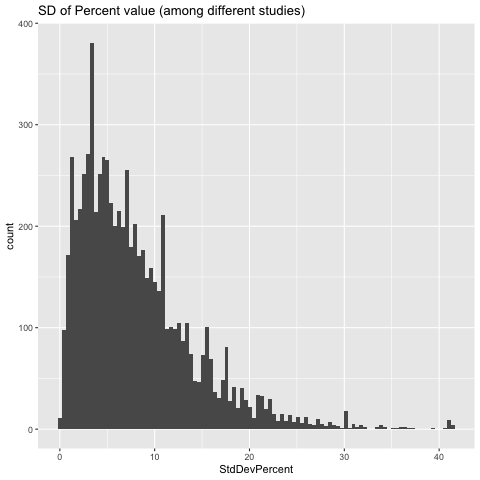
\includegraphics[width=.9\linewidth]{./Plots/rnaseq_perc_sd.png}
\end{center}
\end{document}
